%% abtex2-modelo-include-comandos.tex, v-1.9.5 laurocesar
%% Copyright 2012-2015 by abnTeX2 group at http://www.abntex.net.br/ 
%%
%% This work may be distributed and/or modified under the
%% conditions of the LaTeX Project Public License, either version 1.3
%% of this license or (at your option) any later version.
%% The latest version of this license is in
%%   http://www.latex-project.org/lppl.txt
%% and version 1.3 or later is part of all distributions of LaTeX
%% version 2005/12/01 or later.
%%
%% This work has the LPPL maintenance status `maintained'.
%% 
%% The Current Maintainer of this work is the abnTeX2 team, led
%% by Lauro César Araujo. Further information are available on 
%% http://www.abntex.net.br/
%%
%% This work consists of the files abntex2-modelo-include-comandos.tex
%% and abntex2-modelo-img-marca.pdf
%%

% ---
% Este capítulo, utilizado por diferentes exemplos do abnTeX2, ilustra o uso de
% comandos do abnTeX2 e de LaTeX.
% ---

\externaldocument[I-]{chapter04}
\chapter{Meta-Reasoning for selection}\label{ch:rghs}

% ---
\section{Greedy Heuristic Selection (GHS)}
\noindent
We present a greedy algorithm selection for solving the heuristic subset selection problem while optimizing different objective functions. We consider the following general optimization problem.

\begin{equation}
\underset{\zeta\sp{'}\ \subseteq\ \zeta}{minimize}\ \Psi(\zeta\sp{'}, \nabla)
\label{eq:equationmin}
\end{equation}
%\begin{split}
%\textbf{minimize}_{\zeta\sp{'}\ \subseteq\ \zeta}\Psi(\zeta\sp{'}, \nabla) \\
%\end{split}

Where $\Psi(\zeta\sp{'},\nabla)$ is an objective function we want to minimize for a subset of heuristics $\zeta\sp{'}$ of $\zeta$. We use an algorithm based on the local search we call Greedy Heuristic Selection (\texttt{GHS}) to solve Equation \ref{eq:equationmin} for different functions $\Psi$.

\begin{algorithm}
\SetKwInOut{Input}{Input}
\SetKwInOut{Output}{Output}
\Input{problem $\nabla$, set  of heuristics $\zeta$}
\Output{heuristic subset $\zeta\sp{'} \subseteq \zeta$}

$\zeta\sp{'} \leftarrow \emptyset$\\
%$i\ \leftarrow 0$\\ 
\While {$\Psi(\zeta\sp{'},\nabla)$ can be improved} {
	$h\ \leftarrow\ \argminA_{h \in \zeta}  \Psi(\zeta\sp{'} \cup \{h\}, \nabla)$\\
	$\zeta\sp{'} \leftarrow \zeta\sp{'} \cup \{h\}$\\
	%\If{$\Psi(\zeta_{i-1}\sp{'} \cup \{h\}$ can be improved}{
		%$\zeta_{i}\sp{'} \leftarrow \zeta_{i-1}\sp{'} \cup \{h\}$\\
		%$i++$\\
	%}	
} 
return $\zeta\sp{'}$
\caption{Greedy Heuristic Selection}
\label{alg:ghs_algorithm}
\end{algorithm}

Algorithm \ref{alg:ghs_algorithm} shows \texttt{GHS}. \texttt{GHS} receives as input a problem $\nabla$, a set of heuristics $\zeta$, and it returns a subset $\zeta\sp{'} \subseteq \zeta$. In each iteration \texttt{GHS} greedily selects from $\zeta$ the heuristics $h$ which will result in the largest reduction of the value $\Psi$ (line 3). \texttt{GHS} returns $\zeta\sp{'}$ once the objective function cannot be improved. In other words, the algorithm will halt when adding another heuristic does not improve the objective function.

% --
\section{Minimizing Search Tree Size}
% ---
\noindent
The first objective function $\Psi$ we consider accounts for the number of node generations A$\sp{*}$ performs while solving a given planning problem. The planning problem must be solvable, this means $C\sp{*}$ cannot be infinity. When solving $\nabla$ using the consistent heuristic function $h_{max}(\zeta\sp{'})$  for $\zeta\sp{'} \subseteq \zeta$, A$\sp{*}$ generates a number of nodes that is bounded above by $J(\zeta\sp{'},\nabla)$, defined as,

\begin{equation}
J(\zeta\sp{'},\nabla) = |\{children(s) \in V | f_{max}(s,\zeta\sp{'}) \leq C\sp{*}\}|
\label{eq:eq_size_search_tree_1}
\end{equation}
\begin{equation}
J(\zeta\sp{'},\nabla) = |\{children(s) \in V | h_{max}(s,\zeta\sp{'}) \leq C\sp{*} - g(s)\}|
\label{eq:eq_size_search_tree_2}
\end{equation}

We write $J(\zeta\sp{'})$ or simply $J$ instead of $J(\zeta\sp{'},\nabla)$ whenever $\zeta\sp{'}$ and $\nabla$ are free from the context. What's more, we assume that A$\sp{*}$ expands all nodes $s$ with $f(s) \leq C\sp{*}$ while solving $\nabla$, as shown in Equation \ref{eq:eq_size_search_tree_1}.

\iffalse
We now show that $J(\zeta\sp{'}, \nabla)$ is minimal, for the subset $\zeta\sp{'}$ returned by \texttt{GHS}.
\begin{theorem}
Let the heuristics in $\zeta\sp{'}$ as well as $h \notin \zeta'$ be consistent heuristics. We have that
$J(\zeta\sp{'} \cup \{h\}) \le J(\zeta\sp{'})$.\\
\label{lemma:monotonic}
\end{theorem}
\begin{proof}
Fix $\zeta\sp{'}$ and $h$, then: 
\begin{small}
\begin{align*}
J(\zeta' \cup \{h\})  =&\big| \big\{children(s)  \in V \mid h_{max}(s, \zeta'\cup \{h\}) \le C^* -g^*(s)\big\} \big|\\
J(\zeta' \cup \{h\})  \le&\big| \big\{children(s)  \in V \mid h_{max}(s, \zeta') \le C^* -g^*(s)\big\} \big|\\
J(\zeta' \cup \{h\})  =&J(\zeta')\
\end{align*} 
\end{small}
where the inequality follows from the fact that $h_{max}(s, \zeta'\cup \{h\})\ge h_{max}(s, \zeta')$ for all $s$.
\end{proof}

\begin{corollary}
$J(\zeta, \nabla) \leq J(\zeta', \nabla)$ for any $\zeta' \subseteq \zeta$.
\label{eq:max_optimal}
\end{corollary}

\begin{lemma}
Let $\nabla$ be a planning problem with optimal solution cost $C^*$, $A$  a set of consistent heuristic functions, and $B \subseteq A$. If $J(A, \nabla) < J(B, \nabla)$, then there exists an element $h \in A$ such that $J(B \cup \{h\}, \nabla) < J(B, \nabla)$.
\label{lemma:prop}
\end{lemma}

If $J(A, \nabla) < J(B, \nabla)$, then by definition of $J$ there exists a state $s$ for which $f(s, A) > C^*$ and $f(s, B) \le C^*$. Thus, there must exist a heuristic $h \in A$ such that $h(s) > C^* - g^*(s) \ge h_{max}(s, B)$. Then, $h_{max}(s, B \cup \{h\}) > C^* - g^*(s)$ follows from the definition of $h_{max}$, and consequently $J(B \cup \{h\}, \nabla) < J(B, \nabla)$.

\begin{theorem}
Given a set $\zeta$ of consistent heuristics, \texttt{GHS} returns a subset $\zeta\sp{'}$ of $\zeta$ for which $J(\zeta) = J(\zeta\sp{'})$. 
\label{thm:optimalJ}
\end{theorem}

\begin{proof}
 \texttt{GHS} stops when there is no $h \in \zeta$ such that $J(\zeta\sp{'} \cup h) < J(\zeta\sp{'})$ is true. Thus, $J(\zeta) < J(\zeta\sp{'})$ cannot be true (Lemma~\ref{lemma:prop}). Since $J(\zeta)$ is minimal, $J(\zeta') = J(\zeta)$  (Theorem~\ref{thm:optimalJ})..
\end{proof}
\fi

\section{Minimizing A*'s Running Time}
\noindent
Another objective function $\Psi$ we consider is an approximation of the A$\sp{*}$ running time and is defined as follows.

\begin{equation}
T(\zeta\sp{'}, \nabla) = J(\zeta\sp{'},\nabla) \cdot (t_{h_{max}(\zeta\sp{'})} + t_{gen})\,, 
\label{eq:eq_time_solving}
\end{equation}
\noindent

where, for any heuristic function $h$, the term $t_{h_{max}(\zeta\sp{'})}$ refers to the running time used for computing the $h_{max}$ of any state $s$. We assume that $t_{h_{max}(\zeta\sp{'})}$ to be constant in the state space, which is a reasonable assumption for several heuristics such as \texttt{PDBs}. $t_{gen}$ is the node generation time, which we also assume to be constant.

\iffalse
Next we show that if all $h \in \zeta$ have the same evaluation time $t_{h}$, consequently the subset $\zeta\sp{'}$ \texttt{GHS} returns is guaranteed to have the lowest $T$-value amongst all subsets of size $||\zeta\sp{'}$ or larger.

\begin{theorem}
Let $\zeta$ be a set of consistent heuristics. If $t_{h_{i}} = t_{h_{j}}$ for any $h_{i}, h_{j} \in \zeta$, then \texttt{GHS} yields a subset $\zeta\sp{'}$ of $\zeta$ with $T(\zeta\sp{'}, \nabla) \leq T(\zeta\sp{''}, \nabla)$ for any $\zeta\sp{''} \subseteq \zeta$ with $|\zeta\sp{'}| \leq |\zeta\sp{''}|$
\label{th:theorem_evaluation_time_heuristic}
\end{theorem} 

\begin{proof}
\begin{align}
T(\zeta', \nabla) &= J(\zeta', \nabla) \times (t_{h_{max}(\zeta')} + t_{gen}) \\
&\le J(\zeta', \nabla) \times (t_{h_{max}(\zeta'')} + t_{gen}) \label{eq:step1} \\
&\le J(\zeta'', \nabla) \times (t_{h_{max}(\zeta'')} + t_{gen}) \label{eq:step2} \\
&= T(\zeta'', \nabla) \,.
\end{align}
\end{proof}
Inequality~\ref{eq:step1} follows from $t_{h_{max}(\zeta\sp{'})} \leq t_{h_{max}(\zeta\sp{''})}$ (because $|\zeta\sp{'}| \leq |\zeta\sp{''}|$ and $t_h$ is constant for any $h\in\zeta$). Inequality~\ref{eq:step2} follows from $J(\zeta', \nabla)$ being minimal (Theorem~\ref{thm:optimalJ}).
\fi 
 
\iffalse
In order to compute the running time of A$\sp{*}$ exactly we would also have to account for all nodes evaluated. Specifically, our objective function accounts for the generation time added to the heuristic evaluation time of all nodes generated, not only nodes expanded. In this way, $T(\zeta\sp{'},\nabla)$ is reasonable approximation for A$\sp{*}$'s running time for the heuristic subset selection problem.
\fi

\section{Estimating Tree Size and Running Time}
In  practice \texttt{GHS} uses approximations of $J$ and $T$ instead of their exact values. This is because computing $J$ and $T$ exactly would require solving $\nabla$, and this is what we obviously want to avoid.

We use the Culprit Sampler (\texttt{CS}) introduced by Barley et al., (\citeyear{BarleySantiagoOver}) and the Stratified Sampling (\texttt{SS}) algorithm introduced by Chen (\citeyear{chen1992heuristic}), for computing \textit{\^{J}} and \textit{\^{T}}. Each method has its strengths and weaknesses, which we explore in Chapter \ref{ch:empirical_evaluation}, where we make an empirical comparison of GHS with other approaches. 

Both \texttt{CS} and \texttt{SS} must be able to quickly estimate the values of \textit{\^{J}}$(\zeta\sp{'})$ and \textit{\^{T}}$(\zeta\sp{'})$ for any subset $\zeta\sp{'}$ of $\zeta$ so they can be used in \texttt{GHS}'s optimization process.

\section{Culprit Sampler (CS)}
\noindent
\texttt{CS} is an approach introduced by Barley et al., (\citeyear{BarleySantiagoOver}) and works by running a time-bounded A$\sp{*}$ search while sampling $f$-culprits and $b$-culprits. In this dissertation we use \texttt{CS} to estimate the values of \textit{\^{J}} and \textit{\^{T}}.

\begin{definition}(f-culprit)
Let $\zeta = \{h_{1}, h_{2},...,h_{M}\}$ be a set of heuristics. The f$-$culprit of a node n in an A$\sp{*}$ search tree is defined as the tuple F(n) = $\left\langle f_{1}(n), f_{2}(n),...,f_{M}(n)  \right\rangle$, where $f_{i}(n) = g(n)+h_{i}(n)$. For any n$-$tuple F, the counter $C_{F}$ denotes the number of nodes n in the tree with F(n) = F.
\label{def:def_fculprits}
\end{definition}

\begin{definition}(b-culprit)
Let $\zeta = \{h_{1}, h_{2},...,h_{M}\}$ be a set of heuristics and b a lower bound on the solution cost $\nabla$. The $b$-culprit of a node n in an A$\sp{*}$ search tree is defined as the tuple $B(n) = \left\langle y_{1}(n), y_{2}(n),...,y_{M}(n)\right\rangle$, where $y_{i}(n) = 1$ if g(n) + $h_{i}(n) \leq b$ and $y_{i}(n) = 0$, otherwise.  For any binary $n$-tuple B, the counter $C_{B}$ denotes the number of nodes n in the tree with B(n) = B.
\label{def:def_bculprits}
\end{definition}

\texttt{CS} works by running an A$\sp{*}$ search bounded by a user-specified time limit. Then, \texttt{CS} compresses the information obtained in the A$\sp{*}$ search (i.e., the $f$-values of all nodes expanded according to all heuristics $h$ in $\zeta$) in $b$-culprits, which are later used for computing \textit{\^{J}}. The $f$-culprits are generated as an intermediate step for computing the $b$-culprits, as we explain below. The maximum number of $f$-culprits and $b$-culprits in an A$\sp{*}$ search tree is equal to the number of nodes in the tree expanded by the time-bounded A$\sp{*}$ search. However, in practice the number of $f$-culprits is usually much lower than the number of nodes in the tree. Moreover, in practice, the total number of different $b$-culprits tends to be even lower than the total number of $f$-culprits. Given a planning problem $\nabla$ and a set of heuristics $\zeta$, \texttt{CS} samples the A$\sp{*}$ search tree as follows.

\begin{enumerate}
    \item[1.-] \texttt{CS} runs A$\sp{*}$ using $h_{min}(s,\zeta) = min_{h \in \zeta}h(s)$ until reaching a user-specified time limit. A$\sp{*}$ using $h_{min}$ expands node $n$ if it were to expand $n$ while using any of the heuristics in $\zeta$ individually. For each node $n$ expanded in this time-bounded search we store $n$'s $f$-culprit and its counter.
    \item[2.-] Let $f_{maxmin}$ be the largest $f$-value according to $h_{min}$ encountered in the time-bounded A$\sp{*}$ search described above. We now compute the set $\mathbb{B}$ of $b$-culprits and their counters based on the $f$-culprits and on the value of $f_{maxmin}$. This is done by iterating over all $f$-culprits once.

\end{enumerate}
    
The process described above is performed only once \texttt{GHS}'s execution. The value of \textit{\^{J}}$(\zeta\sp{'},\nabla)$ for any subset $\zeta\sp{'}$ of $\zeta$ if then computed by iterating over all $b$-culprits \textbf{B} and summing up the relevant values of $C_{B}$. The relevant values of $C_{B}$ represent the number of nodes A$\sp{*}$ would expand in a search bounded by $b$ if using $h_{max}(\zeta\sp{'})$. This computation can be written as follows.

\begin{equation}
\textit{\^{J}}(\zeta\sp{'},\nabla) = \sum_{\mathbb{B} \in B}W(B)
\label{eq:eq_comp_w}
\end{equation}

Where $W(B)$ is 0 if there is a heuristic in $\zeta\sp{'}$ whose $y$-value in $B$ is zero (i.e., there is a heuristic in $\zeta\sp{'}$ that prunes all nodes compressed into $B$), and $C_{B}$ otherwise. If the time$-$bounded A$\sp{*}$ search with $h_{min}$ expands all nodes $n$ with $f(n) \leq C\sp{*}$, then \textit{\^{J}}$=J$. In practice, however, our estimate \textit{\^{J}} will tend to be much lower than $J$.

The value of \textit{\^{T}} is computed by multiplying \textit{\^{J}} by the sum of the evaluation time of each heuristic in $\zeta\sp{'}$. The evaluation time of the heuristics in $\zeta\sp{'}$ is measured in a separate process, before executing \texttt{CS}, by sampling a small number of nodes from $\nabla$'s start state.

\section{Stratified Sampling (SS)}
Chen (\citeyear{chen1992heuristic}), presented a method for estimating the search tree size of backtracking search algorithms by using a stratification of the search tree to guide its sampling. We define Chen’s stratification as a type system.

\begin{figure}[htb]
\centering 
\begin{tikzpicture}

% -- center, xdim, ydim
\draw[very thick,cyan] \boundellipse{-2,0}{2}{4};
\draw[very thick,cyan] \boundellipse{6,0}{1}{2};
	
  % First, define nodes
% -- points F  
  
  \draw (-2,3) node[circle, inner sep=0.8pt, fill=cyan, label={{}}] (E) {};  
  \draw (6,1) node[circle, inner sep=0.8pt, fill=cyan, label={{}}] (F) {}; 

  \draw[very thick,cyan, ->>]  (E) .. controls +(5,-3) and +(-4,1).. (F);
  \path  ($(E)+(0,0.2)$) .. controls +(5,-3) and +(-4,1)..  ($(F)+(0,0.2)$) 
     {\foreach \i in {1,...,40} {  coordinate[pos=0.15+0.75*\i/40] (p\i) } };

  \draw (-1,2) node[circle, inner sep=0.8pt, fill=cyan, label={{}}] (A) {};
  \draw[very thick,cyan, ->>]  (A) .. controls +(5,-3) and +(-4,1).. (F);
  \path  ($(A)+(0,0.2)$) .. controls +(5,-3) and +(-4,1)..  ($(F)+(0,0.2)$) 
     {\foreach \i in {1,...,40} {  coordinate[pos=0.15+0.75*\i/40] (p\i) } };
	
  \draw (-3,0) node[circle, inner sep=0.8pt, fill=cyan, label={{}}] (B) {};
  \draw[very thick,cyan, ->>]  (B) .. controls +(5,-3) and +(-4,1).. (F);
  \path  ($(B)+(0,0.2)$) .. controls +(5,-3) and +(-4,1)..  ($(F)+(0,0.2)$) 
     {\foreach \i in {1,...,40} {  coordinate[pos=0.15+0.75*\i/40] (p\i) } };
	
% -- points in G

  \draw (-2,1) node[circle, inner sep=0.8pt, fill=cyan, label={{}}] (C) {};
  \draw (6.5,0) node[circle, inner sep=0.8pt, fill=cyan, label={{}}] (G) {};
  \draw[very thick,cyan, ->>]  (C) .. controls +(5,-3) and +(-4,1).. (G);
  \path  ($(C)+(0,0.2)$) .. controls +(5,-3) and +(-4,1)..  ($(G)+(0,0.2)$) 
     {\foreach \i in {1,...,40} {  coordinate[pos=0.15+0.75*\i/40] (p\i) } };	

\draw (-1,0) node[circle, inner sep=0.8pt, fill=cyan, label={{}}] (D) {};	
\draw[very thick,cyan, ->>]  (D) .. controls +(5,-3) and +(-4,1).. (G);
  \path  ($(C)+(0,0.2)$) .. controls +(5,-3) and +(-4,1)..  ($(G)+(0,0.2)$) 
     {\foreach \i in {1,...,40} {  coordinate[pos=0.15+0.75*\i/40] (p\i) } };	

\draw (-3,-1) node[circle, inner sep=0.8pt, fill=cyan, label={{}}] (H) {};	
\draw[very thick,cyan, ->>]  (H) .. controls +(5,-3) and +(-4,1).. (G);
  \path  ($(C)+(0,0.2)$) .. controls +(5,-3) and +(-4,1)..  ($(G)+(0,0.2)$) 
     {\foreach \i in {1,...,40} {  coordinate[pos=0.15+0.75*\i/40] (p\i) } };
	
% -- X
\draw (-2,-2) node[circle, inner sep=0.8pt, fill=cyan, label={{}}] (J) {};
  \draw (6,-1) node[circle, inner sep=0.8pt, fill=cyan, label={{}}] (X) {};
  \draw[very thick,cyan, ->>]  (J) .. controls +(5,-3) and +(-4,1).. (X);
  \path  ($(C)+(0,0.2)$) .. controls +(5,-3) and +(-4,1)..  ($(G)+(0,0.2)$) 
     {\foreach \i in {1,...,40} {  coordinate[pos=0.15+0.75*\i/40] (p\i) } };

\draw (-2,-3) node[circle, inner sep=0.8pt, fill=cyan, label={{}}] (K) {};
\draw[very thick,cyan, ->>]  (K) .. controls +(5,-3) and +(-4,1).. (X);
  \path  ($(C)+(0,0.2)$) .. controls +(5,-3) and +(-4,1)..  ($(G)+(0,0.2)$) 
     {\foreach \i in {1,...,40} {  coordinate[pos=0.15+0.75*\i/40] (p\i) } };

$\node [xshift=1cm,yshift=2cm] (A) at (-3,3) {Search Space};$

$\node [xshift=1cm,yshift=2cm] (A) at (5,1) {Type System};$
	
\end{tikzpicture}
\caption{Type system and the search space representation.} \label{fig:ss_ts}
\end{figure}

\subsection{Type System}
The type system is calculated based of any property of nodes in the search tree. A common definition is the one that assigns two nodes to the same type if they have the same $f$-value (Lelis et al., \citeyear{lelis2013predicting}). In the Figure \ref{fig:ss_ts} we can see that the type system is a partition of the state space.

\iffalse
A common mistake about type system is to think that it is an abstraction of the state$-$space. Prieditis, (\citeyear{Prieditis93}) defines a state$-$space abstraction as a simplified version of the problem where:
\begin{itemize}
\item The cost of the least$-$cost path between two abstracted states must less than or equal to the cost of the least$-$cost path between the corresponding two states in the original state$-$space.
\item Goal states in the original state$-$space must be goal states in the abstracted state$-$space.
\end{itemize}

The difference between state-space abstractions and type system is that the last one does not have the two requeriments mentioned above. Also, there is not relation between types to argue that the type system can be represented as a graph. Furthermore, the relation between type system and abstractions is that type system can not necessarily used as abstractions, and abstraction always can be used as a type system Prieditis, (\citeyear{Prieditis93}).
\fi

\begin{definition}{Type System}
Let S = (N,E) be a search tree, where N is its set of nodes and  for each n $\in$ N, $\{n\sp{'}|(n,n\sp{'})\ \in\ E \}$ is n's set of child nodes. $TS = \{t_{1},...,t_{k} \}$ is a type system for S if it is a disjoint partitioning of N. If $n\ \in\ N$ and $t\ \in\ TS$ with $n\ \in\ t$, we write $TS(n) = t$.
\end{definition}


According to Lelis et al., (\citeyear{lelis2013predicting}), \texttt{SS} is able to approximate functions of the form $\varphi = \sum_{n \in S}z(n)$, where $z$ is a function assigning a numerical value to a node, consequently $\varphi$ is a numerical property of $S$. For example, if $z(n)=1$ for all $n \in S$, then $\varphi$ is the size of the tree. Instead of summing all the $z$-values from the tree, \texttt{SS} considers  subtrees rooted at nodes of the same type will have equal values of $\varphi$ and only one of each type, chosen at random, is expanded. With input a search tree $S$ and a type system $TS$, \texttt{SS} predicts $\varphi$ in the following way: First, the search tree is sampled, returning the set of $\emph{representative-weight}$ pairs, with one such pair for every unique type seen during sampling. Second, in the pair $\left\langle s,w \right\rangle$ in $A$ for type $t \in TS$, $n$ is the unique node of type $t$ that was expanded during search and $w$ is an estimate of the number of nodes of type $t$ in the tree. Finally, $\varphi$ is then approximated by $\hat{\varphi}$, defined as, $\hat{\varphi} =  \sum_{\left\langle s,w \right\rangle \in A}w \times z(n)$.

\iffalse
According to Lelis et al., (\citeyear{lelis2013predicting}), \texttt{SS} is a general method for approximating any function of the form $\varphi = \sum_{n \in S}z(n)$, where $z$ is any function assigning a numerical value to a node.  $\varphi$ represents a numerical property of the search tree rooted at $n\sp{*}$. For instance, if $z(n)=1$ for all $n \in S$, then $\varphi$ is the size of the tree. Instead of traversing the entire tree and summing all $z-$values, \texttt{SS} assumes subtrees rooted at nodes of the same type will have equal values of $\varphi$ and only one node of each type, chosen randomly, is expanded. This is the key to $\texttt{SS}$'s efficiency since the search trees of practical interest have far too many nodes to be examined exhaustively. Given a search tree $S$ and a type system $TS$, \texttt{SS} estimates $\varphi$ as follows. First, it samples the tree and returns a set $A$ of $\emph{representative-weight}$ pairs, with one such pair for every unique type seen during sampling. In the pair $\left\langle s,w \right\rangle$ in $A$ for type $t \in TS$, $n$ is the unique node of type $t$ that was expanded during search and $w$ is an estimate of the number of nodes type $t$ in the tree. $\varphi$ is then approximated by $\hat{\varphi}$, defined as, $\hat{\varphi} =  \sum_{\left\langle s,w \right\rangle \in A}w \times z(n)$. 
\fi


By making $z(n) = |children|$ for all $n \in S$ \texttt{SS} prooduces an estimate $\hat{J}$ of $J$. Similarly to our approach with \texttt{CS}, we obtain $\hat{T}$ by multiplying $\hat{J}$ by the sum of heuristic evaluation time and generation time.


\begin{algorithm}
\SetKwInOut{Input}{Input}
\SetKwInOut{Output}{Output}
\Input{root $n\sp{*}$ of a tree and a type system $TS$, upper bound $d$, heuristic function $h$}
\Output{an array of sets $A$, where $A[i]$ is the set of (node, weight) pairs $<s,w>$ for the nodes $n$ expanded at level $i$.}

$A[0] \leftarrow \{\left\langle  s\sp{*},1 \right\rangle \}$

$i \leftarrow 0$

\While{A[i] is not empty} {
	\For{each element $\left\langle s,w \right\rangle$ in $A[i]$} {
		\For{each child $\hat{n}$ of n} {
			\If{$g(\hat{n}) + h(\hat{n}) \leq d$} {
				\If{$A[i+1]$ contains an element $\left\langle n\sp{'}, w\sp{'} \right\rangle$ with $TS(n\sp{'}) = TS(\hat{n})$} {
				$w\sp{'} \leftarrow w\sp{'} + w$\\ 
				with probability $w/w\sp{'}$, replace $\left\langle n\sp{'}, w\sp{'} \right\rangle$ in $A[i+1]$ by $\left\langle \hat{n},w\sp{'} \right\rangle$
				} \Else {	
					insert new element $\left\langle \hat{n},w \right\rangle$	 in $A[i+1]$
				}
			}
		}
	}
	$i \leftarrow i + 1$
}
\caption{SS, a single probe}
\label{alg:ss_algorithm}
\end{algorithm}

In \texttt{SS} the types are required to be partially ordered: a node's type must be strictly greater than the type of its parent. This can be guaranteed by adding the depth of a node to the type system and then sorting the types lexicographically. That is why in our implementation of \texttt{SS} types at one level are treated separately from types at another level by the division of $A$ into groups $A[i]$, where $A[i]$ is the set of $\emph{representative-weight}$ pairs for the types encountered at level $i$. If the same type occurs on differente levels the occurrences will be treated as if they were different types $-$ the depth of search is implicitly included into all of our type systems.

Algorithm \ref{alg:ss_algorithm} shows \texttt{SS} in detail. Representative nodes from $A[i]$ are expanded to get representative nodes for $A[i+1]$ as follows. $A[0]$ is initialized to contain only the root of the search tree to be probed, with weight 1 (Line 1). In each iteration (Lines 4 through 11), all nodes in $A[i]$ are expanded. The children of each node in $A[i]$ are considered for inclusion in $A[i+1]$ if their $f$-value do not exceed an upper bound $d$ provided as input to \texttt{SS}. If a child $\hat{n}$ has a type $t$ that is already represented in $A[i+1]$ by another node $n\sp{'}$, then a $merge$ action on $\hat{n}$ and $n\sp{'}$ is performed. In a merge action we increase the weight in the corresponding $\emph{representative-weight}$ pair of type $t$ by the weight $w(n)$ of $\hat{n}$'s parent $n$ (from level $i$) since there were $w(n)$ nodes at level $i$ that are assumed to have children of type $t$ at level $i+1$. $\hat{n}$ will replace $n\sp{'}$ according to the probability shown in Line 9. Chen (\citeyear{chen1992heuristic}), proved that this probability reduces the variance of the estimation. Once all the states in $A[i]$ are expanded, we move to the next iteration.

One run of the \texttt{SS} algorithm is called a $probe$. Chen (\citeyear{chen1992heuristic}), proved that the expected value of $\hat{\varphi}$ converges to $\varphi$ in the limit as the number of probes goes to infinity. As Lelis et al., (\citeyear{lelis2014estimating}) showed, \texttt{SS} is not able to detect duplicated nodes in its sampling process. As a result, since A$\sp{*}$ does not expanded duplicates, \texttt{SS} usually overestimates the actual number of nodes A$\sp{*}$ expands. Thus, in the limit, as the number of probes grows large, \texttt{SS}'s prediction converges to a number which  is likely to overestimate the A$\sp{*}$ search tree size. We test empirically whether \texttt{SS} is able to allow \texttt{GHS} to make good subset selects despite being unable to detect duplicated nodes during sampling.

Similarly to \texttt{CS}, we also define a time-limit to run \texttt{SS}. We use \texttt{SS} with an iterative-deepening approach in order to ensure an estimate of $\hat{J}$ and $\hat{T}$ before reaching the time limit. We set the upper bound $d$ to the heuristic value of the start state and, after performing $p$ probes, if there is still time, we increase $d$ to twice its previous value. The values of $\hat{J}$ and $\hat{T}$ is given by the prediction produced for the last $d$-value in which \texttt{SS} was able to sample from.

\texttt{SS} must also be able to estimate the values of $\hat{J}(\zeta\sp{'})$ and $\hat{T}(\zeta\sp{'})$ for any subset $\zeta\sp{'}$ of $\zeta$. This is achieved by using \texttt{SS} to estimate $b$-culprits (see Definition \ref{def:def_bculprits}) instead of the search tree size directly. Similarly to \texttt{CS, SS} used $h_{min}$ of the heuristics in $\zeta$ to decide when to prune a node (see Line 6 of Algorithm \ref{alg:ss_algorithm}) while sampling. This ensures that \texttt{SS} expands a node $n$ if A$\sp{*}$ employing at least one of the heuristics in $\zeta$ would expand $n$ according to bound $d$. The $C_{B}$ counter of each $b$-culprit $B$ encountered during $SS$'s probe is given by,

\begin{equation}
C_{B} = \sum_{\left\langle n,w \right\rangle \in A \wedge B(n) = B}w
\label{eq:eq_CB}
\end{equation}

We recall that to compute $B(n)$ for node $n$ one needs to define a bound $b$. Here we use the bound $d$ used by \texttt{SS}. The average value of $C_{B}$ across $p$ probes is used to predict the search tree size for a given subset $\zeta\sp{'}$. As explained for \texttt{CS}, this can be done by traversing all $b$-culprits once.

\if false

\section{8-tile-puzzle Case Using type system}
\noindent
In this dissertation we use type system based only in heuristics.\cite{lelis2013predicting} use the type system where two nodes have the same type if they have the same heuristic value.

\begin{figure}[htb]
\centering
\begin{forest}
 [\usebox\myboxc \hspace*{1.4in} \usebox\myboxb]
\end{forest}
\caption{The heuristic value is the position of the empty tile in a specific state.} \label{fig:type_system}
\end{figure}

Let's explain how type system works through an example. The problem of 8-tile-puzzle in the Figure \ref{fig:type_system}, the center tile is labeled with the letter \texttt{M}, the corners labeled with \texttt{C} and the mediums with \texttt{E}. For this problem, we can define the type system based on the position of the empty tile regarding the position of the empty tile in the goal state. For this case, two nodes $n$ and $n\sp{'}$ would be of the same type if $n$ and $n\sp{'}$ have the empty tile with the same letter and with the same distance to the empty tile of the goal state.

In the Figure \ref{fig:empty_space_ts}, each row represent a type. The first board shows the empty tile in the center with distance to the empty tile in the goal state equal to 2. The shortest path to get to the empty tile in the goal state would be doing: down$-$left or right$-$down. Which both moves represent the same cost. Then, the type would be (2,\texttt{M}). In the next board, the empty tile is in the left top, and use the letter \texttt{C}. The minimum distance is 4 because to get the goal empty tile is necessary to do: down$-$down$-$right$-$right or right$-$right$-$down$-$down, etc. So the type would be (4, \texttt{C}). In the next board, there are two tiles that have the same type, because both have the same letter \texttt{M} with distance equal to 3. Then, both have the type (3,E). The fourth row have two boards with the same type, because both have the same letter \texttt{C} with distance equal to 2. Then, both have the type (2, \texttt{C}). The fifth row have two boards with the same type, because both have the same letter \texttt{E} with distance equal to 1. Then, both have the type (1, \texttt{E}). In the last row the empty tile is in the goal empty tile. So, the distance is zero and the letter is \texttt{C}. The type would be (0, \texttt{C}).

% print types
\begin{figure}[htb]
\centering
\begin{forest}
 [\usebox\myboxcenter]
 $\node [xshift=1cm,yshift=2cm] (A) at (2,0) {(2, M)};$
\end{forest}

\begin{forest}
 [\usebox\myboxcornerone]
 $\node [xshift=1cm,yshift=2cm] (A) at (2,0) {(4, C)};$
\end{forest}

\begin{forest}
 [\usebox\myboxmediumleft \hspace*{0.2in} \usebox\myboxmediumup]
 $\node [xshift=1cm,yshift=2cm] (A) at (4,0) {(3, E)};$
\end{forest}

\begin{forest}
 [\usebox\myboxcornerthree \hspace*{0.2in} \usebox\myboxcornertwo]
 $\node [xshift=1cm,yshift=2cm] (A) at (4,0) {(2, C)};$
\end{forest}

\begin{forest}
 [\usebox\myboxmediumdown \hspace*{0.2in} \usebox\myboxmediumright]
 $\node [xshift=1cm,yshift=2cm] (A) at (4,0) {(1, E)};$
\end{forest}

\begin{forest}
 [\usebox\myboxcornerfour]
 $\node [xshift=1cm,yshift=2cm] (A) at (2,0) {(0, C)};$
\end{forest}
\caption{Each row has one or two states that represent the same type.} \label{fig:empty_space_ts}
\end{figure}

\fi

\section{SS step by step}
\noindent
% -- Explaining Stratified Sampling
In the Figure \ref{fig:ts_search_tree}, we can see an example of an \texttt{SS} run. Thus, nodes have different types if they have different colors or are in different levels of the search tree.

In the level 1, we have the root node, and their $w$ is initialized with one. In the level 2 three nodes are generated by the root node. The nodes in level 2 have the following types: red and blue, and each node receive the same $w$ from their parent. Since we assume that nodes of the same type root subtrees of the same size, then only one node of each type needs to be expanded. In level 2 there are two nodes with the red type. In that way, we choose randomly one of them to expand. Let us suppose we choose the right red node. Then, we have to update the number of nodes with the red type by summing their $w$-values, since both nodes of the red type have $w = 1$, then we sum the $w$ resulting in $w=2$.

\begin{figure}[htb]
\centering
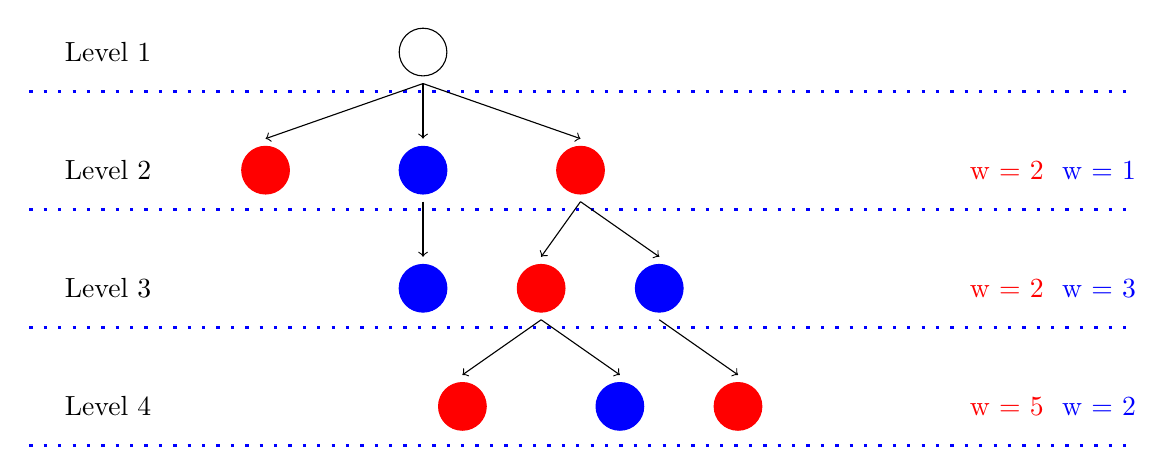
\begin{tikzpicture}

\draw[very thick,blue,loosely dotted] (-2,0) -- (12,0);
\draw[very thick,blue,loosely dotted] (-2,-1.5) -- (12,-1.5);
\draw[very thick,blue,loosely dotted] (-2,-3) -- (12,-3);
\draw[very thick,blue,loosely dotted] (-2,-4.5) -- (12,-4.5);

\node [xshift=1cm,yshift=2cm] (A) at (-2,-1.5) {Level 1};
\node [xshift=1cm,yshift=2cm] (A) at (-2,-3) {Level 2};
\node [xshift=1cm,yshift=2cm] (A) at (-2,-4.5) {Level 3};
\node [xshift=1cm,yshift=2cm] (A) at (-2,-6) {Level 4};

% -- level 1
\draw[black,fill=white] (3,0.5) circle (2ex);

% -- level 2
\draw[red,fill=red] (1,-1) circle (2ex);
\draw[blue,fill=blue] (3,-1) circle (2ex);
\draw[red,fill=red] (5,-1) circle (2ex);

% -- level 3
\draw[blue,fill=blue] (3,-2.5) circle (2ex);
\draw[red,fill=red] (4.5,-2.5) circle (2ex);
\draw[blue,fill=blue] (6,-2.5) circle (2ex);

% -- level 4
\draw[red,fill=red] (3.5,-4) circle (2ex);
\draw[blue,fill=blue] (5.5,-4) circle (2ex);
\draw[red,fill=red] (7,-4) circle (2ex);

% -- draw arrows
\draw[->] (3,0.1) -- (1,-0.6);
\draw[->] (3,0.1) -- (3,-0.6);
\draw[->] (3,0.1) -- (5,-0.6);

\draw[->] (3,-1.4) -- (3,-2.1);

\draw[->] (5,-1.4) -- (4.5,-2.1);
\draw[->] (5,-1.4) -- (6,-2.1);

\draw[->] (4.5,-2.9) -- (3.5,-3.6);
\draw[->] (4.5,-2.9) -- (5.5,-3.6);

\draw[->] (6,-2.9) -- (7,-3.6);

\node [xshift=1cm,yshift=2cm] (A) at (10,-3) {\textcolor{red}{w = 2 } \textcolor{blue}{w = 1}};
\node [xshift=1cm,yshift=2cm] (A) at (10,-4.5) {\textcolor{red}{w = 2 } \textcolor{blue}{w = 3}};
\node [xshift=1cm,yshift=2cm] (A) at (10,-6) {\textcolor{red}{w = 5 } \textcolor{blue}{w = 2}};
\end{tikzpicture}
\caption{Search tree using type system} \label{fig:ts_search_tree}
\end{figure}

Let's suppose that nodes in level 2 are expanded. The blue node generates one node of the blue type and the red node generates two nodes with the following types: red and blue. To compute the $w$-values of the nodes at level 3 we do the following. The $w$-value of nodes of the red type is computed by summing up the $w$-values of all parents that generated a node of the red type at level 3. In this case only one node at level 2 generated a node of the red type at level 3. Since this node has a $w$-value of 2, then \texttt{SS} estimates that there is 2 nodes of the red type at level 3 (red type's $w$-value). Two nodes at level 2 generate a blue node at level 3, thus we have to sum their $w$-values, resulting in $w = 2 + 1 = 3$ for blue nodes.

\iffalse
The question that raises here is how many nodes are generated in the Level 3. To answer this question, we only have to apply a simple multiplication between each type and their respectively weight $w$ and then sum all the nodes with the same type. For Level 3 the answer would be: $1 \times \textcolor{blue}{blue} + 2 \times \textcolor{red}{red} + 2 \times \textcolor{blue}{blue}$. Therefore, in Level 3 we will have 2 nodes of the red type and 3 nodes of the blue type. This process continues until reaching the bottom of the tree.

In the Level 3 the $w$ of the node blue would have the same $w$ of their father. Their father has $w = 1$, then the child has $w = 1$. The $w$ of the red node and blue node would be 2. Once the $w$ has been updated for each node in the Level 3,	 we apply the \texttt{SS}'s assumption again. There are two nodes with type blue. Then, we choose randomly one of them to update their $w$. Let's suppose we choose the right blue type and their updated $w$ would be 3 because 1 from the left blue type plus 2 from the right blue type.

Now, we have to expand the nodes in the Level 3. Let's imaging that they are expanded in the following way: The red node generates two nodes of types red and blue from left to right and the blue node generates one of type red. How many nodes would be generated at Level 4, then? The answer is: $2 \times \textcolor{red}{red} + 3 \times \textcolor{red}{red} + 2 \times \textcolor{blue}{blue}$. As a result, in the Level 4, we will have five nodes of type red and two nodes of type blue.
\fi

Finally, the number of nodes expanded in the search tree is obtained summing all $w$ plus one (the root node). In summary, the number of nodes expanded in the search tree would be $ 15 + 1 = 16$. 

If we run the algorithm again maybe in level 2 instead of choosing the right red node we could choose the left red node and the nodes generated in level 3 would be different. As a consequence, the number of nodes generated could be higher or lower than we have now. In other words, in each probe of the algorithm could result in a different value of the estimated tree size. In order to obtain accurate estimates of the search tree size one has to usually perform several probes of \texttt{SS} and average the results.

\clearpage